\documentclass[tikz,border=10pt]{standalone}
\usepackage{amsmath}
\usetikzlibrary{arrows.meta}

\begin{document}
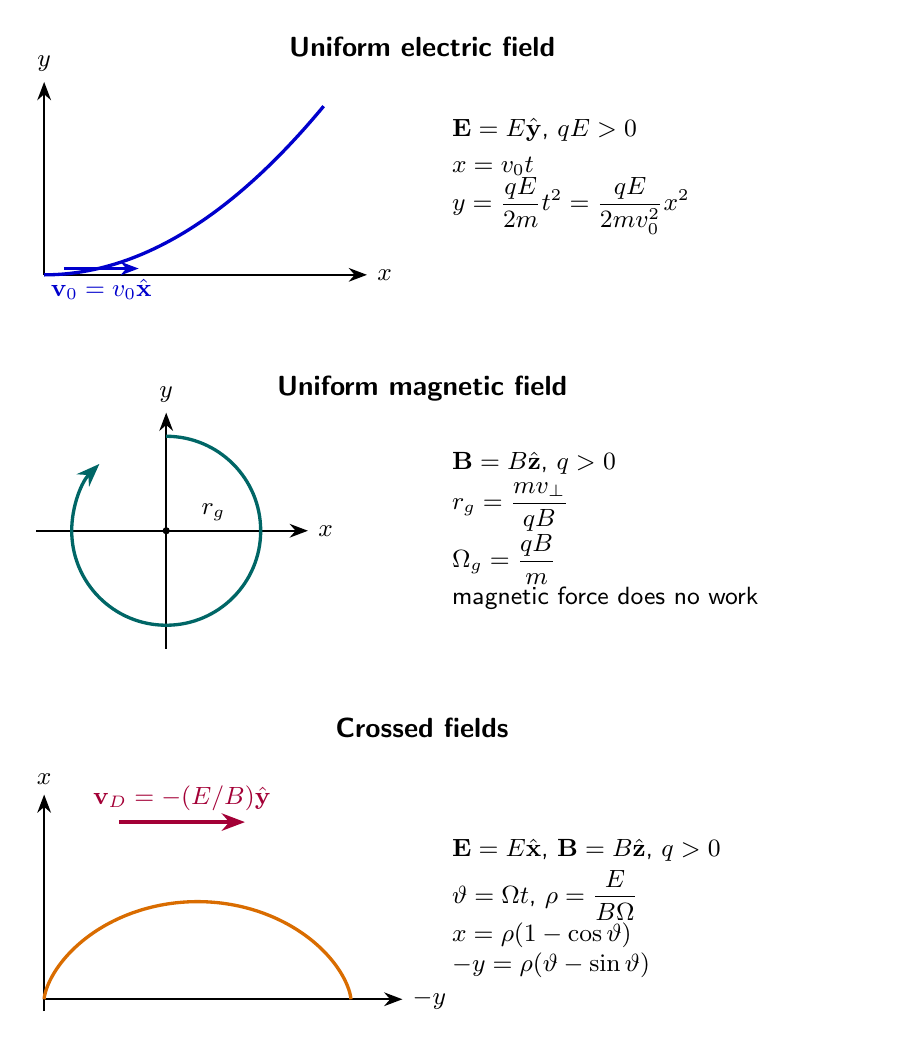
\begin{tikzpicture}[
  >=Stealth,
  thick,
  font=\sffamily\small,
  note/.style={align=left,text width=5.2cm}
]
  % Uniform electric field: x=v_0 t, y=qEt^2/(2m), with qE>0.
  \begin{scope}[yshift=9.2cm]
    \node[font=\sffamily\bfseries] at (4.8,2.9) {Uniform electric field};
    \draw[->] (0,0)--(4.1,0) node[right] {$x$};
    \draw[->] (0,0)--(0,2.45) node[above] {$y$};
    \draw[blue!80!black,very thick,domain=0:3.55,samples=100]
      plot (\x,{0.17*\x*\x});
    \draw[->,blue!80!black] (.25,.08)--(1.2,.08)
      node[midway,below] {$\mathbf v_0=v_0\hat{\mathbf x}$};
    \node[note,anchor=west] at (5.05,1.25) {
      $\mathbf E=E\hat{\mathbf y}$, $qE>0$\\[2pt]
      $x=v_0t$\\
      $y=\dfrac{qE}{2m}t^2
       =\dfrac{qE}{2mv_0^2}x^2$
    };
  \end{scope}

  % Uniform magnetic field: q>0 gives clockwise motion for B along +z.
  \begin{scope}[yshift=4.7cm]
    \node[font=\sffamily\bfseries] at (4.8,3.05) {Uniform magnetic field};
    \draw[->] (-.1,1.25)--(3.35,1.25) node[right] {$x$};
    \draw[->] (1.55,-.25)--(1.55,2.75) node[above] {$y$};
    \draw[teal!80!black,very thick,->]
      (1.55,2.45) arc[start angle=90,end angle=-225,radius=1.20];
    \fill (1.55,1.25) circle (1.3pt);
    \draw[dashed] (1.55,1.25)--(2.75,1.25)
      node[midway,above] {$r_g$};
    \node[note,anchor=west] at (5.05,1.25) {
      $\mathbf B=B\hat{\mathbf z}$, $q>0$\\[2pt]
      $r_g=\dfrac{mv_\perp}{qB}$\\
      $\Omega_g=\dfrac{qB}{m}$\\
      magnetic force does no work
    };
  \end{scope}

  % Crossed fields: exact cycloid for rest initial data and q>0.
  \begin{scope}
    \node[font=\sffamily\bfseries] at (4.8,3.45) {Crossed fields};
    \draw[->] (0,0)--(4.55,0) node[right] {$-y$};
    \draw[->] (0,-.15)--(0,2.6) node[above] {$x$};
    \draw[orange!85!black,very thick,domain=0:6.283,samples=140]
      plot ({0.62*(\x-sin(\x r))},{0.62*(1-cos(\x r))});
    \draw[->,purple!85!black,very thick] (.95,2.25)--(2.55,2.25)
      node[midway,above] {$\mathbf v_D=-(E/B)\hat{\mathbf y}$};
    \node[note,anchor=west] at (5.05,1.15) {
      $\mathbf E=E\hat{\mathbf x}$,
      $\mathbf B=B\hat{\mathbf z}$, $q>0$\\[2pt]
      $\vartheta=\Omega t$,
      $\rho=\dfrac{E}{B\Omega}$\\
      $x=\rho(1-\cos\vartheta)$\\
      $-y=\rho(\vartheta-\sin\vartheta)$
    };
  \end{scope}
\end{tikzpicture}
\end{document}
